\section{Discrete Wavelet Transform}

\subsection{One dimensional DWT}

\begin{figure}
    \centering
    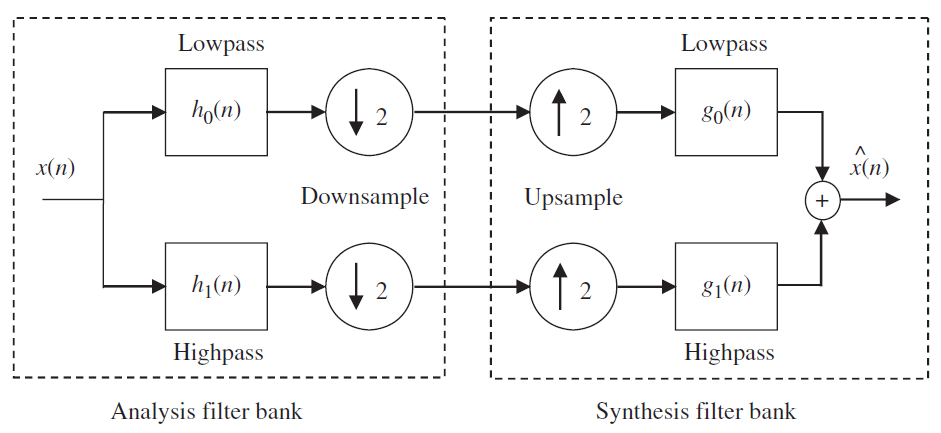
\includegraphics[scale=0.5]{dwt_1d_anal_synth.png}
    \caption{1-D DWT, two-band wavelet analysis and synthesis filter banks \cite{jpeg_suite}}
    \label{fig:dwt_1d_anal_synth}
\end{figure}

The linear convolution (filtering) of sequences $x(n)$ and $h(n)$ is defined as in equation \ref{eq:convolution}:
\begin{equation}
    y(n)=\sum_{m=-\infty}^{\infty}x(m)h(n-m)
\label{eq:convolution}
\end{equation}
The one dimensional discrete wavelet transform can be depicted as successive applications (convolutions) of
one selected pair of high and low-pass filters. The output of such application is then followed
by downsampling by the factor of two. For example, it can be achieved by discarding samples with
odd indices after each of filtering operation. It is better visualized in the Figure \ref{fig:dwt_1d_anal_synth} \cite{jpeg_suite}.
The pair of low and high-pass filters is known as analysis filter bank in the encoding process.
In the signal decoding process it is featured as a synthesis filter bank. The decoding step requires
using the inverse of discrete wavelet transform.

Take into consideration a one dimensional signal $x(n) = \{55, 234, 70, 21, 88, 37\}$. It can be better
understood as values of pixels in a part of the grayscale image row. It is followed with a pair of low
and high-pass filters designated by $h_{0}(n)$ and $h_{1}(n)$ respectively. An example of such pair is
a lowpass filter $h_{0}(n) = \{-1, 2, 6, 2, -1\}/8$ and a high-pass filter $h_{1}(n) = \{-1, 2, -1\}/2$. They are both
symmetric and consist of only integer operations. Such pair can be presented in the notation of (5, 3) filter bank.
This convention indicates that the length of lowpass filter is five and the length of high-pass filter is three.
In fact the analysis filter bank presented here was firstly proposed by LeGall and Tabatabai in 1988 and
is used in the JPEG 2000 standard for lossless compression of images. The filtering operation has to
be defined at the signal boundaries. Therefore, the one dimensional signal is extended in both directions.
The Part 1 of the JPEG 2000 standard requires symmetrical extension to be performed in such case \cite{jpeg_suite}.
After applying the required symmetrical padding the signal is extended to
$x(n) = \{21, 70, 234, 55, 55, 234, 70, 21, 88, 37, 37, 88, 21, 70\}$. Then, the low-pass filter is applied
resulting in $x'_{0}(n) = \{197.25, 75.5, 98.375, 67.125, 45.375\}$ and the high-pass one which results in
$x'_{1}(n) = \{44.75, -85.75, 29, 12.75, -29.5\}$.

\begin{figure}
    \centering
    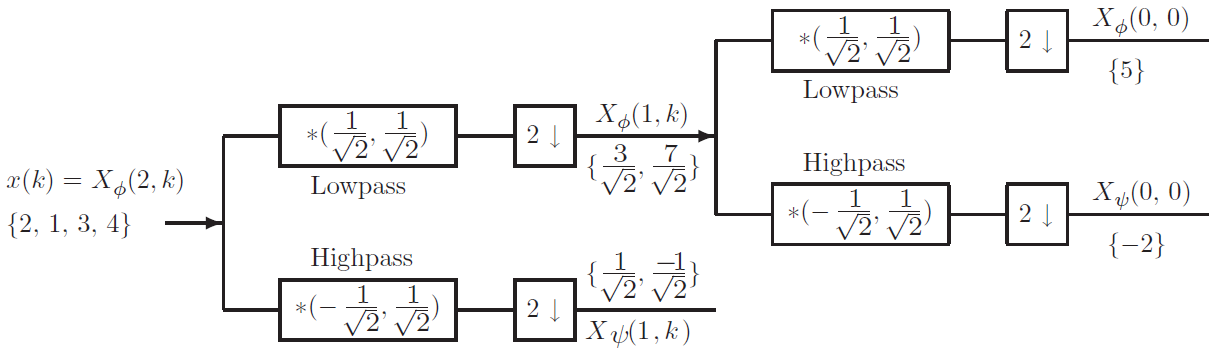
\includegraphics[scale=0.45]{dwt_1d_2_level.png}
    \caption{Computation of a 2-level 4-point DWT using a two-stage two-channel Haar analysis filter bank \cite{dwt_impl}}
    \label{fig:dwt_1d_2_level}
\end{figure}

The next example shows how to compute the two levels of discrete wavelet transform. To speed up the process
no padding option is chosen this time which makes it non-compliant with the JPEG 2000 standard.
The filter used here is the most basic one, i.e. Haar analysis filter bank. It is the first wavelet
from the Daubechies wavelet family. The calculation process is visualized in the Figure \ref{fig:dwt_1d_2_level} \cite{dwt_impl}.

The input is chosen as 4-point signal $X_{\phi}(2, k) = \{2, 1, 3, 4\}$. This notation emphasizes the fact
that it is approximation of the input at scale 2. The so called scaling coefficients (or in other term
approximation at scale 1) $X_{\phi}(1, k)$ are computed by convolving the input $x(k)$ with the low-pass
Haar filter impulse response $l(k) = \{1/\sqrt{2}, 1/\sqrt{2}\}$. In the next step there is downsampling
by a factor of 2 applied. The output of convolution has five values. The middle three from these fives 
correspond to cases where both the given input values overlap with the impulse response. As it was described
earlier, the odd values are preserved in the downsampling process. In a result first and third value of these
three middle ones are the approximation output $X_{\phi}(1, k)$. In the similar way, the detail coefficients
at scale 1 $X_{\psi}(1, k)$ are computed. The input $x(k)$ is convolved with the high-pass filter impulse
response $h(k) = \{-1/\sqrt{2}, 1/\sqrt{2}\}$. Then the downsampling by factor of 2 is performed.
Note that only only approximation output $X_{\phi}(1, k)$ of the first stage goes to the second one.
The $X_{\phi}(0, 0)$ and $X_{\psi}(0, 0)$ are calculated accordingly at the end of the second stage \cite{dwt_impl}.

\subsection{Two dimensional DWT}

The idea of using lowpass filter is the preservation of low frequencies of a signal while trying
to eliminate or at least attenuate the high frequencies. In a result the output signal is the blurred
version of the original one. Therefore, the operating principle of the high-pass filter is completely
opposite. As a result of applying such filter, the high frequencies of the signal are preserved and
the low ones are discarded or at least diminished. The output is a signal consisting of edges, textures
and other details \cite{jpeg_suite}.

\begin{figure}
    \centering
    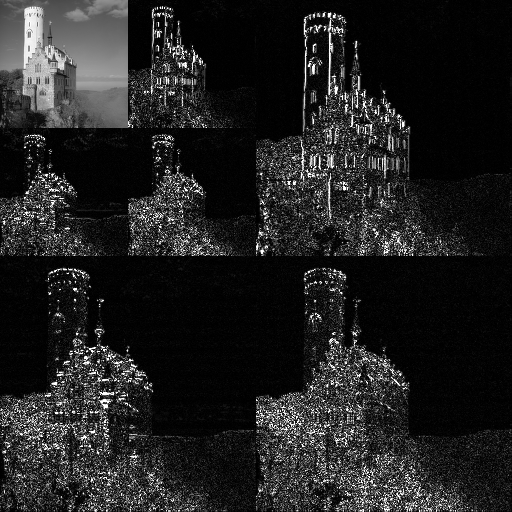
\includegraphics[scale=0.7]{dwt_2d_example_wiki.png}
    \caption{2D DWT applied 2 times to an exemplary image \cite{dwt_example_wiki}}
    \label{fig:dwt_2d_example_wiki}
\end{figure}

There is presented an example of the effects of the two dimensional discrete wavelet transform on the Figure \ref{fig:dwt_2d_example_wiki}.
The DWT used here is compliant with the Part 1 of the JPEG2000 standard. The number of DWT stages presented in this  
example is equal to two. Two dimensional discrete wavelet transform applied first time to the original image
yields four same sized sub-images. The LL layer (upper left sub-image) is an approximation of the image and contains the low frequencies.
This layer is once more transformed in the next stage. The LH layer (upper right sub-image) preserves high frequencies from the rows of the image.
As a result vertical lines and details (brightness) can be seen in the produced sub-image. On the other hand, the HL layer (bottom left)
contains high frequencies from the columns of the image. The horizontal details and lines can be noticed there.
Lastly, the HH layer (bottom right) preserves the diagonal lines \cite{dwt_example_wiki}.

\begin{figure}
    \centering
    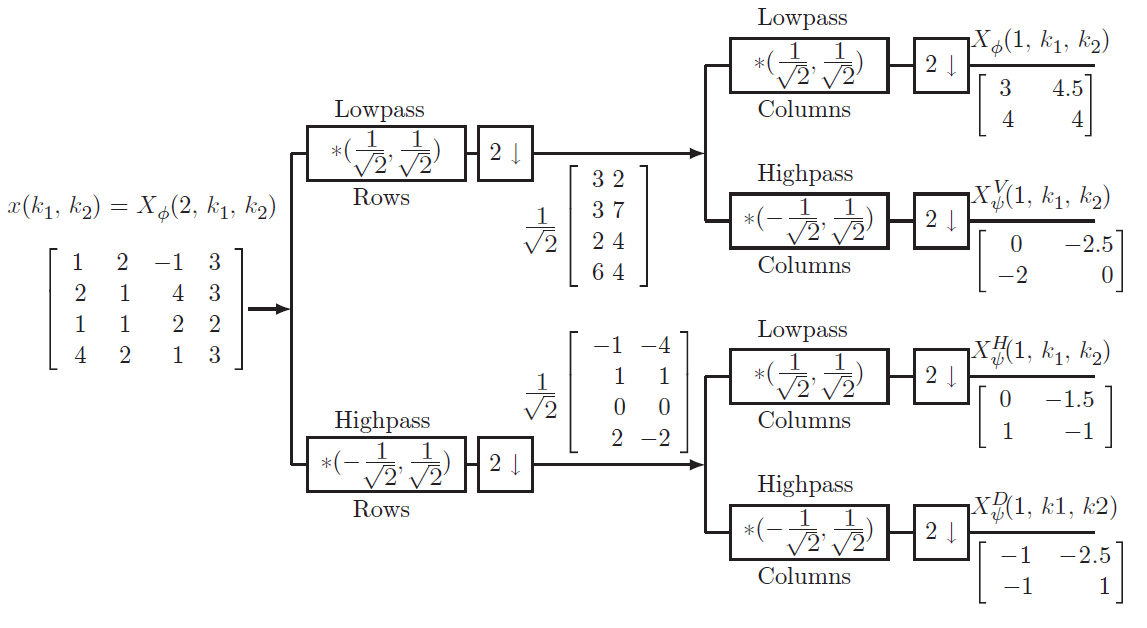
\includegraphics[scale=0.45]{dwt_2d_1_level.png}
    \caption{Computation of a 1-level 4 $\times$ 4 2-D Haar DWT using a two-stage filter bank \cite{dwt_impl}}
    \label{fig:dwt_2d_1_level}
\end{figure}

The process of computing a 1 level two dimensional discrete wavelet transform with usage of
two-stage analysis Haar filter bank is shown in Figure \ref{fig:dwt_2d_1_level}. Coefficients $\mathbf{X}_{\phi}$
are calculated as a result of lowpass filtering and downsampling to each row of the two dimensional
data. Next, similar process process, i.e. lowpass convolution and downsampling is applied to each column of
resulting data. The rest of coefficients is obtained in very similar fashion to the previous ones.
Coefficients $\mathbf{X}^{H}_{\psi}$ are calculated by applying high-pass filtering and downsampling to each row of the
2-D data $\mathbf{x}$ and then followed by applying sequence of low-pass filtering and downsampling to each
column of the resulting data. Coefficients $\mathbf{X}^{V}_{\psi}$ are obtained by applying low-pass filtering
and then downsampling to each column of the resulting data. Lastly, coefficients $\mathbf{X}^{D}_{\psi}$ are
obtained by applying high-pass filtering and downsampling to each row of the 2-D data $\mathbf{x}$ followed by
applying high-pass filtering and downsampling to each column of the resulting data. In the next stage of more
complex DWT calculating process only the coefficients $\mathbf{X}_{\phi}$ are taken into consideration \cite{dwt_impl}.

\subsection{DWT features summary}

\begin{itemize}
    \item In a nutshell, the discrete wavelet transform is a set of bandpass filters. Usually it is implemented
    with the usage of low and high-pass filters recursively.
    \item The computational complexity of computing the DWT in the best case is linear, i.e. $O(N)$.
    \item The first approach to implement the DWT efficiently is evaluation of the required convolutions
    with the usage of the polyphase filter structure.
    \item The second approach is factorization of the polyphase matrix into a product of a set of sparse matrices.
    \item The two dimensional discrete wavelet transform (with separable filters) is usually computed by the row-column method.
    One dimensional DWT of all the columns is computed at first. Then the 1-D DWT of all the resulting
    rows is calculated. The order of the computation in the row-column method can be swapped. The result remains the same.
    \item Additional memory of approximate half the size of the given data is required in the some implementations of the DWT.
    However, there also exist methods of computing DWT in-place which do not require additional memory. 
    \item Data reordering is required for an in-place computation of the DWT.
    \item Data expansion problem can occur due to the finite length of the data in the implementation of the asymmetric filters.
    \item Symmetric filters provide linear phase response and an effective solution to the border problem \cite{dwt_impl}.
\end{itemize}

\section{Part 2 of the JPEG 2000} \label{sec:part2_jpeg2000}

% Part2 in details
% write down different filters and basic ones

\subsection{Introduction}

Many ideas have been emerging as the JPEG 2000 was developed. These concept were full of
value-added capabilities. However, they were not that important to be gone through the time-consuming
ISO standardization process. The Part 1 (ISO/IEC, 2004a) of the standard, i.e. Core coding system, 
was originally published in 2000. There was a need to create additional parts to include
missing features. The Part 2 of the standard, published as ISO/IEC 15444-2 or ITU Recommendation
T.801 (ISO/IEC, 2004b), contains multiple such extensions. There is present group of rather small
additions that could not merit entire documents of their own. In the Part 1 Core of JPEG 2000
standard decoders are supposed to handle all of the code-stream functionality. The Part 2
is different from first one in this aspect. It is a collection of options that can be
implemented on demand to meet very specific requirements of the given market. Moreover,
sections within an extension annex can be implemented separately. For example, subsets
of extended file format JPX can be used on their own. Therefore, some features of the Part 2
may be present in the wide spectrum of JPEG 2000 applications while the other ones can be
less common in the decoders \cite{jpeg_suite}.

As it was shown in the previous paragraph, the extensions present in the Part 2 consist of 
very different set of topics that can modify or add some features to the Part 1 JPEG 2000 compliant 
processing chain. Some tools can result in the compression efficiency improvement. Others can
ameliorate the visual appearance of compressed images. Another group of extensions can modify
or extend some functionalities in the other ways. The list of the major topics is presented below \cite{jpeg_suite}.
\newline \newline Compression efficiency:
\begin{itemize}
    \item Variable DC offset (VDCO) - Annex B
    \item Variable scalar quantization (VSQ) - Annex C
    \item Trellis coded quantization (TCQ) - Annex D
    \item Extended visual masking - Annex E
    \item Arbitrary wavelet decomposition - Annex F
    \item Arbitrary wavelet transform kernel - Annexes G and H
    \item Multiple component transform - Annex J
    \item Nonlinear point transform - Annex K \cite{jpeg_suite}
\end{itemize}
\hfill \break Functionalities:
\begin{itemize} 
    \item Geometric manipulation - Annex I
    \item Single-sample overlap (SSO/TSSO) - Annex I
    \item Precinct-dependent quantization - Amendment 1
    \item Extended region of interest - Annex L
    \item Extended file format/metadata (JPX) - Annexes M and N
    \item Extended capabilities signaling - Amendment 2 \cite{jpeg_suite}
\end{itemize}

\subsection{Arbitrary Decomposition} \label{sec:arbitrary_decomposition}

In the Part 1 of the JPEG 2000 standard there is only one wavelet decomposition structure allowed.
This wavelet is called Mallat dyadic decomposition. Such decomposition is a good first choice
to be applied across a wide spectrum of images. However, other ones can improve the quality of the image
over specialized classes of the applications. The other effect of applying such decompositions are
unequal reductions in the horizontal and vertical dimensional of reduced resolution extracts \cite{jpeg_suite}.

\begin{figure}
    \centering
    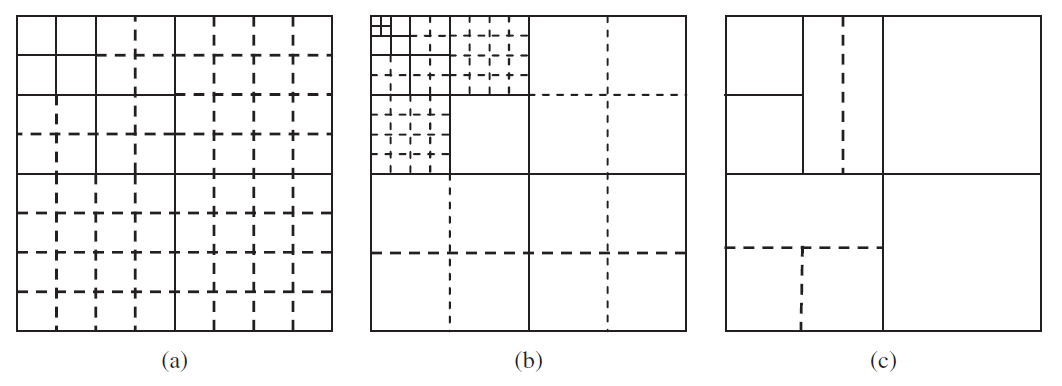
\includegraphics[scale=0.45]{part_2_decomp_examples.png}
    \caption{Some examples of decomposition compliant with the Part 2 \cite{jpeg_suite}}
    \label{fig:part_2_decomp_examples}
\end{figure}

Other decomposition styles can be found in the wavelet literature. They include the full packet
tree processing and some of its derivatives. The applied packet decomposition derivatives
can outperform the solution from Part 1 of the JPEG 2000 standard in some applications.
For instance, they come crucial at maintaining regular fine-grain texture. Moreover,
the applications that require processing synthetic aperture radar images can benefit
from using this extension. The US Federal Bureau of Investigation actively uses a 500 ppi
fingerprint compression standard, i.e. WSQ (CJIS, 1997). The decomposition is specialized
for the characteristics of fingerprint imagery at 500 dpi \cite{jpeg_suite}.

Some of these decomposition can be seen of the Figure \ref{fig:part_2_decomp_examples}.
Resolution decomposition is depicted as solid lines. Dashed lines represent extra sublevel
decomposition. On the first example, i.e. image $(a)$, there is available full packet decomposition
with such parameters: NL = 3: Ddfs = 111, Doads = 321, Dsads = all 1s. The next picture
illustrates FBI decomposition wit specified parameters: NL = 5: Ddfs = 11111, Doads = 2321,
Dsads = 11101111111111111. The last image is juts an arbitrary example \cite{jpeg_suite}.

The prespecified decomposition structures are not the only feature of this extension.
Wavelet packet analysis can be also used to design custom decompositions for specific images
or some types of images. It was implemented in these papers \cite{entropy_algos},
\cite{wavelet_packet} and \cite{adaptive_wavelet}. Such applications often start with
a large decomposition tree. Then, they tend to locate a good decomposition based upon
specified optimization metric \cite{jpeg_suite}.

\subsection{Arbitrary Wavelet Transforms} \label{sec:arbitrary_wavelet_transform}

\begin{table}
    \centering
    \caption{Analysis and synthesis filter taps for the floating-point Daubechies (9, 7) filter bank}
    \label{tab:anal_synth_97i}
\begin{tabular}{ccc}
    \toprule
    n         & Low-pass, $h_{0}(n)$ & Low-pass, $g_{0}(n)$ \\
    \midrule
    $0$       & +0.602949018236360  & +1.115087052457000  \\
    $\pm 1$   & +0.266864118442875  & +0.591271763114250  \\
    $\pm 2$   & -0.078223266528990  & -0.057543526228500  \\
    $\pm 3$   & -0.016864118442875  & -0.091271763114250  \\
    $\pm 4$   & +0.026748757410810  &                     \\
    \bottomrule
\end{tabular}

\bigskip
\bigskip


\begin{tabular}{cc}
    \toprule
    n         & High-pass, $h_{1}(n)$ \\
    \midrule
    $-1$      & +1.115087052457000   \\
    $-2, 0$   & -0.591271763114250   \\
    $-3, 1$   & -0.057543526228500   \\
    $-4, 2$   & +0.091271763114250   \\
              &                      \\
    \bottomrule
\end{tabular}
\quad
\begin{tabular}{cc}
    \toprule
    n        & High-pass, $g_{1}(n)$ \\
    \midrule
    $1$      & +0.602949018236360   \\
    $0, 2$   & -0.266864118442875   \\
    $-1, 3$  & -0.078223266528990   \\
    $-2, 4$  & +0.016864118442875   \\
    $-3, 5$  & +0.026748757410810   \\
    \bottomrule
\end{tabular}
\end{table}

\begin{table}
    \centering
    \caption{Analysis and synthesis filter taps for the integer (5, 3) filter bank}
    \label{tab:anal_synth_53r}
\begin{tabular}{ccc}
    \toprule
    n         & Low-pass, $h_{0}(n)$ & Low-pass, $g_{0}(n)$ \\
    \midrule
    $0$       & +0.75  & +1    \\
    $\pm 1$   & +0.25  & +0.5  \\
    $\pm 2$   & -0.125 &       \\
    \bottomrule
\end{tabular}

\bigskip
\bigskip


\begin{tabular}{cc}
    \toprule
    n         & High-pass, $h_{1}(n)$ \\
    \midrule
    $-1$      & +1   \\
    $-2, 0$   & -0.5 \\
              &      \\
    \bottomrule
\end{tabular}
\quad
\begin{tabular}{cc}
    \toprule
    n        & High-pass, $g_{1}(n)$ \\
    \midrule
    $1$      & +0.75  \\
    $0, 2$   & -0.25  \\
    $-1, 3$  & -0.125 \\
    \bottomrule
\end{tabular}
\end{table}

The Part 1 of the JPEG 2000 standard specifies only two possible wavelet transforms.
The reversible one (5-3R, Table \ref{tab:anal_synth_53r}) and the irreversible one
(9-7I, Table \ref{tab:anal_synth_97i}). As it was stated before, both
are required to perform periodic symmetric signal extension at the boundaries.
It is similar case to the Mallat dyadic decomposition in terms of generic implementation.
These filters can compress quite well a wide set of image types. However, certain image
classes can be compressed more efficiently with other types of wavelets. Such a flexibility
is allowed in the Part 2 compliant applications. The range of wavelet transforms is broadened
to include not only the wider range of whole-sample symmetric ones but also half-sample and
generic nonsymmetric ones. Such ability to handle generic filters makes JPEG 2000 standard
a powerful research tool, together with supporting more than niche compression applications \cite{jpeg_suite}.

\section{Parallelism in computer architecture}

The parallelism as general term can be simply understood as two or more separate activities
that appear to happen at the same time. It is not only computer science specific abstraction
but also natural part of life. For instance a person can drive a car and simultaneously
talk on the phone or one person can have a walk, while the other one is riding bike.
However, the computer science aspect of parallelism is the interesting part in this paper.
It can be depicted as single system performing multiple independent tasks at the same time
rather than one after the other \cite{cpp_concurrency}. Multitasking operating systems have been
in usage for many years. However, running multiple applications was firstly done only by context switching.
The situation has been a little bit different in the server industry. High-end machines with multiple processors
have been available there for years making utilization of the real parallelism possible.
In recent years there is observed increase of personal computers capable of running multiple tasks
in similar manner \cite{cpp_concurrency}.

Nowadays, there is a trend in producing increasing amount of processors in multicore solutions by chip manufacturers.
There can be found 16 or even more processor cores on a single chip. Following this way is easier
for improving performance over strengthening single core solutions. Therefore, multicore desktop
computers and even embedded devices are growing share in the market. In the past, it was possible
for programmers to get their application run faster without doing anything. Such situation
was linked with the growing computation power within new generation for single core solutions. 
The situation is quite different at the present time. If a software has to take advantage of
increasing computing power, one has to design and utilize concurrent run of multiple tasks \cite{cpp_concurrency}.

There are two approaches of utilizing concurrency in terms of performance. The most obvious one
is just to divide a single task into separate parts. Then, such subtasks can be run in parallel
reducing the total execution time of the program. This approach is called ``task parallelism''.
Despite sounding rather straightforward, such operation can become a complex process.
Especially whether there exist many dependencies between the separated parts. Such division
can be applied in two different ways. The first one is connected with processing, i.e.
one thread executes certain part of the given algorithm while the other ones perform operations
at the different part. The other way is connected strictly with the data. Each thread
performs the same operation on different parts of the given data. The latter approach is called
data level parallelism \cite{cpp_concurrency}.

There exists quite notable subgroup of algorithms which are basically ready to be parallelized.
They are often referred as ``embarrassingly parallel'', ``naturally parallel'' or
``conveniently concurrent'' \cite{cpp_concurrency}. Such algorithms are especially good in terms
of scalability properties. As the number of available hardware resources, i.e. threads
increases, the parallelism level in the algorithm is trivial to match. However, if there exist
parts of the algorithm which are not easy to parallelize, one has to divide the algorithm
into a fixed number of tasks. Therefore such application becomes not scalable one \cite{cpp_concurrency}.

The another way to use parallelism for improving performance is to employ existing concurrent
solutions to solve bigger issues. This approach can be depicted as processing 2, 5 or 10 files at
given time instead of just one. Although it seems like another application of data level parallelism,
there is different focus in performing such operation on sets of data concurrently.
The amount of time needed to process one chunk of data is still the same. However, more data
can be processed in the same amount of time. Unfortunately, there are limits on this specific
approach as well. Moreover, there are cases where such attitude can be nonbeneficial at all.
In the end, the increase in throughput which comes from this specific approach makes
new things possible, e.g. increased resolution in video processing where different areas
of the picture can be processed at the same time \cite{cpp_concurrency}.
    

\section{Known solutions}

\subsection{Part 1 compliant applications} \label{sec:part_1}

There are multiple solutions that implement features from the Part 1 of the JPEG 2000 standard.
The OpenJPEG library is an example of such application. It is open-source solution developed to
promote wider usage of this standard. The main part of this project is the codec compliant with
the Part 1 of the JPEG 2000 standard. Moreover, the OpenJPEG library integrates other parts
of the standard \cite{jpeg_suite}. Few of them can be seen on the list below:

\begin{itemize}
    \item from the Part 2: handling the JP2 boxes and extended multiple component
    transforms for multi and hyperspectral imagery.
    \item from the Part 3: MJ2 (Motion JPEG 2000).
    \item from the Part 11: JPWL (JPEG 2000 Wireless).
    \item OPJViewer, a GUI based tool for visualization of the J2K (extension used for storing
    code-stream JPEG 2000 data), JP2 (standard JPEG 2000 file extension), JPWL and MJ2 files.
    \item OPJIndexer, a code-stream indexer to view information about the headers and packets localization.
    This tool is also capable of reading the rate-distortion contribution of each packet to the image \cite{jpeg_suite}.
\end{itemize}

The OpenJPEG library is written in the C programming language and released under the BSD license.
The main targets of this software are desktop platforms, i.e. Win32, Unix and Mac OS platforms.
The Communications and Remote Sensing Lab (TELE) of the Catholic University of Louvain (UCL)
is the main developer group of this library. CS company and CNES is the supporting side.
Some of the modules are maintained by the Digital Signal Processing Lab (DSPLab) of the University
of Perugia, mainly the JPWL and OPJViewer. \cite{jpeg_suite}.

Another example of Part 1 compliant application is the JasPer. This computer software project is aimed
to create reference implementation of the standard codec. The project was started by the Image Power Inc.
and the University of British Columbia back in the 1997. As OpenJPEG JasPer is written in the C programming language.
There are some sample applications available in the codebase. They can come in handy while testing the codec. 
JasPer is currently released publicly under the MIT license. The library is a component of several notable
software projects. It includes but is not limited to netpbm, ImageMagick and KDE. In series of the JPEG 2000
compression tests conducted in 2004 JasPer turned out to be the top performing solution, closely followed by
IrfanView and Kakadu. The disadvantage of this implementation is its time performance. In the same tests
JasPer was the slowest software. However, it is a feature as this codec was designed to be used as reference
in non performance-critical systems.

There is one more notable implementation of the Part 1, i.e. Grok. It is open-sourced software released under
the GNU Affero General Public License (AGPL) version 3 license. Its design aims to provide stable, high
performant and low memory using solution. The function responsible for decoding process (grk\_decompress)
is currently over 0.5 the speed of the Kakadu software. Moreover, Grok supports fast sub-tile decoding
to standard output for png, jpeg, bmp, pnm and raw formats. This library supports both TLM and PLT code stream markers
for fast single-tile and sub-tile decoding of large tiled images. The support of meta-data formats such as
XML, IPTC, XMP and ICC profiles is also included. There is also initial version of Part 15 implementation
(High Throughput JPEG 2000) available. The final version of this solution should be ten times faster over
the original Part 1 of the JPEG 2000 standard.

\subsection{Kakadu} \label{sec:kakadu}

Kakadu is not only a complete implementation of the JPEG 2000 standard Part 1 but also an application
that supports Part 2 and Part 3 in a significant amount of features. The software was originally developed
by David Taubman of the University of New South Wales (UNSW) in Australia. The author is also noticeably
known for being the designer of EBCOT, i.e. the core coding component of JPEG 2000. The name of this library
comes from ``Kakadu National Park'' which is located in the Northern Territory of Australia \cite{jpeg_suite}. Licensing
is more advanced in comparison to solutions mentioned in \fullref{sec:part_1}. There are separate licensing
schemes for research, commercial and demonstration-only applications.

The Kakadu software framework is widely adopted in the substantial range of JPEG 2000 products. The few examples
are Apple's Quicktime v6 for MAC, Yahoo's Messenger, Google Earth and Internet Archive \cite{jpeg_suite}. 
Features that can be realized thanks to Kakadu's implementation by the named beforehand solutions include live video
and products for geospatial imagery such as MicroImages TNT. Moreover, this framework is used in medical imaging applications,
interactive image rendering applications, remote browsing of large collection and images, digital cinema applications
and the other fields that require compression and decompression of JPEG 2000 images and videos \cite{jpeg_suite}.

Kakadu is considered as a comprehensive, heavily optimized and fully compliant software toolkit for JPEG 2000
developers. There are multiple features available that make runtime execution so flawless. Multithreaded
processing is supported in such way that makes the most of parallel processing resources, i.e. multiple CPUS,
multicore CPUs and hyperthreading \cite{jpeg_suite}. Compiler intrinsic functions are utilized to manually
vectorize processing of data in processor's pipeline. Moreover, Kakadu comes with built-in thread scheduler.
Such implementation enables possibility of utilizing all computational resources close to 100\%.
In a 2007 the JasPer library was outperformed by Kakadu in terms of speed.

Supported features of Part 2 include arbitrary wavelet transform kernels and general multicomponent transforms.
The Kakadu library offers extensive support for interactive mode of client–server applications. It is done
thanks to the implementation of the most notable features from the JPIP (JPEG 2000 Internet Protocols) standard \cite{jpeg_suite}.

\subsection{Reversible denoising and lifting steps with step skipping}

Methods such as reversible denoising and lifting based color component transformation aim to improve
overall quality of image compression. Color space transformation in reversible manner is required
by the lossless image compression framework used in the JPEG 2000 standard. The undesirable side effect
of such transformation is contamination of transformed components with noise from other ones.
Therefore, the compression ratio of given image is substantially diminished \cite{denoising}.

The work in this specific paper is aimed to remove correlation without increasing the noise.
Therefore, a reversible denoising and lifting step (RDLS) was proposed. The RDLS integrates
usage of denoising filters into lifting step. New image component transformation is a result
of applying RDLS to color space transformation. The main feature of this operation is
being ``reversible despite involving the inherently irreversible denoising'' \cite{denoising}.

The main targets using application of RDLS to the RDgDb color space transformation with
simple denoising filters are the JPEG-LS, JPEG 2000 and JPEG XR lossless modes of the
standard algorithms.
The images which have native optical resolution of acquisition devices benefit the most
from this application. Improvement in terms of compression ratios is the most visible
in subset of images which unmodified color space transformation either improved or worsened
ratios in comparison to the untransformed image. On the average improvement is between
5\% and 6\% for such specific images. However, things differ for images from ``standard
test-sets'' resulting in the improvement only up to 2.2\% \cite{denoising}.

Another application of the RDLS (reversible denoising and lifting step) is described
in the paper \cite{entropy}. New method of using ``hybrid transform'' was introduced there.
The main input to that paper was discrete wavelet transform using custom prediction
mechanism. Although simple prediction is considered to be ineffective when combined with DWT,
the application of modified discrete wavelet transform using RLDS with step skipping is able to
take advantages of its strengths. The usage of heuristics and estimation of entropy resulted
in making described transform ``image-adaptive'' \cite{entropy}.

The data set used for experiments in the presented paper contained 247 non-photographic and
499 photographic images. As a result it was found that described approach using combination
of RDLS with step skipping, DWT and prediction turned out to be effective. The prediction
mechanism allowed to double the JPEG 2000 compression ratio improvements made by using only RDLS.
Compression schemes with various tradeoffs were proposed due to fact that for some images
applying prediction instead of DWT could be more beneficial. The compression ratios of non-photographic
and photographic images improved by 30.9\% and 1.2\%, respectively, in comparison to solution
compliant with Part 1 of the JPEG 2000 standard. The cost was in the increase of compression
time by 2\% and breaking mentioned before compliance. Greater ratio improvements were claimed to
be possible with greater cost in runtime performance \cite{entropy}.

\subsection{Skipping Selected Steps of DWT Computation}

The other method of improving image compression, i.e. bitrates of lossless JPEG 2000 is skipping
selected steps of discrete wavelet computation (SS-DWT). At the first phase of implementing
this particular method fixed SS-DWT variants were employed. Then, heuristic was employed to select
from the mentioned before variants best one for certain image \cite{skipping_dwt}.

The experiments on diverse set of images resulted in the improvement of bitrates vastly of
non-photographic images. ``The entropy estimation of encoding effects'' was used to select the most
feasible variant of applied fixed SS-DWT. It is especially important from the practical standpoint
as time execution of such application is reduced. ``Such compression scheme is compliant with the Part 2
of the JPEG 2000 standard as opposed to the general SS-DWT case'' \cite{skipping_dwt}.

The average improvement in terms of bitrate was around 5\% for the entire test-set. Moreover,
the time needed to perform compression of the image was only 3\% great than the part 1 of the JPEG 2000
compliant variant. However, the results are quite different across the set of photographic and non-photographic
images. The first ones are improved on average by 0.5\% while the latter by 14\%. The heuristic can
be further exploited to perform more modifications and result with improvement of bitrate up to 17.5\%.
These extra modifications include ``skipping the steps based on the actual bitrate rather than the
estimated one and applying reversible denoising and lifting steps to SS-DWT''. However it is achieved with
great time penalty \cite{skipping_dwt}.
Furthermore, it has been evaluated that applying the fixed skipped steps discrete wavelet
transform (fixed SS-DWT) variants with the lossless compression compliant with the Part 2
of JPEG 2000 standard can provide another improvements \cite{practical_dwt}.
